\documentclass[aspectratio=169,10pt]{beamer}

% -----------------------------------------------------------------------------
% Theme & VinUniversity Branding Palette
% -----------------------------------------------------------------------------
\usetheme{Madrid}
\usecolortheme{whale}

\usepackage{fontspec}
\usepackage{amsmath,amssymb,amsfonts}
\usepackage{booktabs}
\usepackage{graphicx}
\usepackage{tikz}
\usepackage{xcolor}
\usepackage{multicol}
\usepackage{tcolorbox}

% VinUniversity Official Colors: Deep Navy & Gold Accent
\definecolor{vinNavy}{RGB}{0, 43, 73}       % #002B49 Primary VinUni Navy
\definecolor{vinGold}{RGB}{197, 160, 89}    % #C5A059 VinUni Gold
\definecolor{vinDarkGold}{RGB}{160, 120, 50}
\definecolor{vinSlate}{RGB}{30, 41, 59}
\definecolor{vinLightBg}{RGB}{248, 250, 252}
\definecolor{vinCoral}{RGB}{225, 29, 72}     % Crimson Red #E11D48
\definecolor{vinGreen}{RGB}{16, 185, 129}   % Emerald Green #10B981

\setbeamercolor{palette primary}{bg=vinNavy,fg=white}
\setbeamercolor{palette secondary}{bg=vinNavy!90!black,fg=white}
\setbeamercolor{palette tertiary}{bg=vinGold,fg=vinNavy}
\setbeamercolor{structure}{fg=vinNavy}
\setbeamercolor{titlelike}{parent=palette primary}
\setbeamercolor{frametitle}{bg=vinNavy,fg=white}

\setbeamercolor{block title}{bg=vinNavy,fg=white}
\setbeamercolor{block body}{bg=vinNavy!6!white,fg=vinSlate}
\setbeamercolor{block title alerted}{bg=vinCoral,fg=white}
\setbeamercolor{block body alerted}{bg=vinCoral!6!white,fg=vinSlate}
\setbeamercolor{block title example}{bg=vinGold!90!black,fg=white}
\setbeamercolor{block body example}{bg=vinGold!10!white,fg=vinSlate}

\setbeamertemplate{navigation symbols}{}
\setbeamertemplate{footline}[frame number]

% -----------------------------------------------------------------------------
% Title Information with VinUniversity Affiliation
% -----------------------------------------------------------------------------
\title[\textbf{SR-CFA | VinUniversity}]{\Large \textbf{Lựa Chọn Kênh Cảm Biến sEMG Rải Rác}}
\subtitle{\large Bằng Trọng Số Giải Thích Ổn Định (SR-CFA) Không Suy Giảm Độ Chính Xác}
\author[\textbf{Ta et al. | VinUni}]{\textbf{Minh-Tri Ta}$^{1}$, \textbf{Hoang-Khang Phan}$^{1}$, \textbf{Le-Giang Tran}$^{1,*}$}
\institute[VinUniversity]{\small $^{1}$Trường Đại học VinUniversity (VinUniversity), Hà Nội, Việt Nam\\$^{*}$Tác giả liên hệ / Báo cáo Nghiên cứu Chuyên đề Y sinh \& AI}
\date{\footnotesize Báo cáo Phương pháp Luận \& Kết quả Thực nghiệm}

\begin{document}

% -----------------------------------------------------------------------------
% Slide 1: Title Slide
% -----------------------------------------------------------------------------
\begin{frame}
    \begin{center}
        {\color{vinGold}\footnotesize \textbf{VINUNIVERSITY $\bullet$ COLLEGE OF ENGINEERING \& COMPUTER SCIENCE}}\\[0.15cm]
        {\color{vinNavy}\LARGE \textbf{Stability-Regularized Cross-Fitted Attribution (SR-CFA)}}\\[0.1cm]
        {\color{vinNavy!80}\normalsize Phương pháp Lựa chọn Cảm biến sEMG Rải rác không Suy giảm Độ chính xác}\\[0.25cm]
        \tcbset{colback=vinNavy!5,colframe=vinGold,width=0.88\textwidth,halign=center}
        \begin{tcolorbox}
            \small \textbf{Nhóm Tác giả:} Minh-Tri Ta, Hoang-Khang Phan, Le-Giang Tran\\
            \footnotesize \textit{VinUniversity, Gia Lâm, Hà Nội, Việt Nam}
        \end{tcolorbox}
    \end{center}
\end{frame}

% -----------------------------------------------------------------------------
% Slide 2: The Big Picture & Practical Paradox
% -----------------------------------------------------------------------------
\begin{frame}{1. Bức Tranh Toàn Cảnh \& Nghịch Lý Kỹ Thuật Chi Giả Đeo}
    \begin{columns}[T]
        \begin{column}{0.48\textwidth}
            \begin{block}{\textbf{Tiềm năng HD-sEMG Mật độ cao (16+ kênh)}}
                \footnotesize
                \begin{itemize}
                    \item Ghi nhận chi tiết xung điện thế cơ bắp (MUAP).
                    \item Phân biệt chính xác \textbf{16 cử chỉ ngón tay/cổ tay}.
                    \item Độ chính xác phòng thí nghiệm thường $> 90\%$.
                \end{itemize}
            \end{block}
            \vspace{0.1cm}
            \begin{alertblock}{\textbf{Rào cản khi đưa vào Ổ cắm Chi giả (Socket)}}
                \footnotesize
                \begin{itemize}
                    \item \textbf{Không gian chật hẹp:} Khó lắp nhiều điện cực tiếp xúc da.
                    \item \textbf{Hao pin \& Tỏa nhiệt:} Mạch khuếch đại đa kênh gây nóng.
                    \item \textbf{Độ trễ thời gian thực:} Bắt buộc xử lý $< 100\text{ ms}$.
                \end{itemize}
            \end{alertblock}
        \end{column}
        
        \begin{column}{0.49\textwidth}
            \begin{exampleblock}{\textbf{Mục tiêu Cốt lõi của Nghiên cứu}}
                \footnotesize
                \textbf{Lựa chọn Cảm biến Rải rác (Sparse Sensor Selection)}:\\
                Tìm số lượng kênh \textbf{tối thiểu $k^*$} sao cho:
                \begin{enumerate}
                    \item \textbf{Không suy giảm độ chính xác:} Hoạt động ngang ngửa mảng đầy đủ 16 kênh.
                    \item \textbf{Dùng ngay cho người mới (Subject-Independent):} Không bắt người dùng phải đo đạc hiệu chuẩn lại từ đầu.
                    \item \textbf{Bền vững theo ngày:} Không bị phế khi tháo ra đeo lại sau 1--2 tuần (donning/doffing).
                \end{enumerate}
            \end{exampleblock}
        \end{column}
    \end{columns}
\end{frame}

% -----------------------------------------------------------------------------
% Slide 3: Three Critical Traps in Literature
% -----------------------------------------------------------------------------
\begin{frame}{2. Ba "Cái Bẫy" Chí Mạng trong Các Nghiên Cứu Trước}
    \begin{columns}[T]
        \begin{column}{0.32\textwidth}
            \begin{alertblock}{\textbf{Bẫy 1: Rò rỉ Dữ liệu\\(Data Leakage)}}
                \scriptsize
                \begin{itemize}
                    \item \textbf{Sai lầm:} Lấy dữ liệu của người test để chuẩn hóa hoặc xếp hạng chọn kênh.
                    \item \textbf{Hậu quả:} Báo cáo độ chính xác ảo $>95\%$, nhưng khi gặp người lạ ngoài đời thật thì sụt giảm $25\text{--}35\%$.
                \end{itemize}
            \end{alertblock}
        \end{column}
        
        \begin{column}{0.32\textwidth}
            \begin{alertblock}{\textbf{Bẫy 2: Trọng số XAI bị Loạn\\(Multicollinearity)}}
                \scriptsize
                \begin{itemize}
                    \item \textbf{Sai lầm:} Các điện cực gần nhau phát tín hiệu tương tự nhau.
                    \item \textbf{Hậu quả:} Thuật toán giải thích (TreeSHAP) chia điểm bấp bênh, mỗi người một phách, không chọn được layout cố định.
                \end{itemize}
            \end{alertblock}
        \end{column}
        
        \begin{column}{0.32\textwidth}
            \begin{alertblock}{\textbf{Bẫy 3: Chọn Kênh Cảm tính\\(Heuristic Guessing)}}
                \scriptsize
                \begin{itemize}
                    \item \textbf{Sai lầm:} Nhìn đồ thị bằng mắt thường rồi tự phán $k=4$ kênh là đủ.
                    \item \textbf{Hậu quả:} Thiếu kiểm định thống kê toán học; thực tế $k=4$ làm giảm sút nghiêm trọng khả năng điều khiển chi giả.
                \end{itemize}
            \end{alertblock}
        \end{column}
    \end{columns}
\end{frame}

% -----------------------------------------------------------------------------
% Slide 4: End-to-End Workflow Architecture
% -----------------------------------------------------------------------------
\begin{frame}{3. Kiến Trúc Tổng Thể Quy Trình Thực Nghiệm (5 Giai Đoạn)}
    \begin{center}
        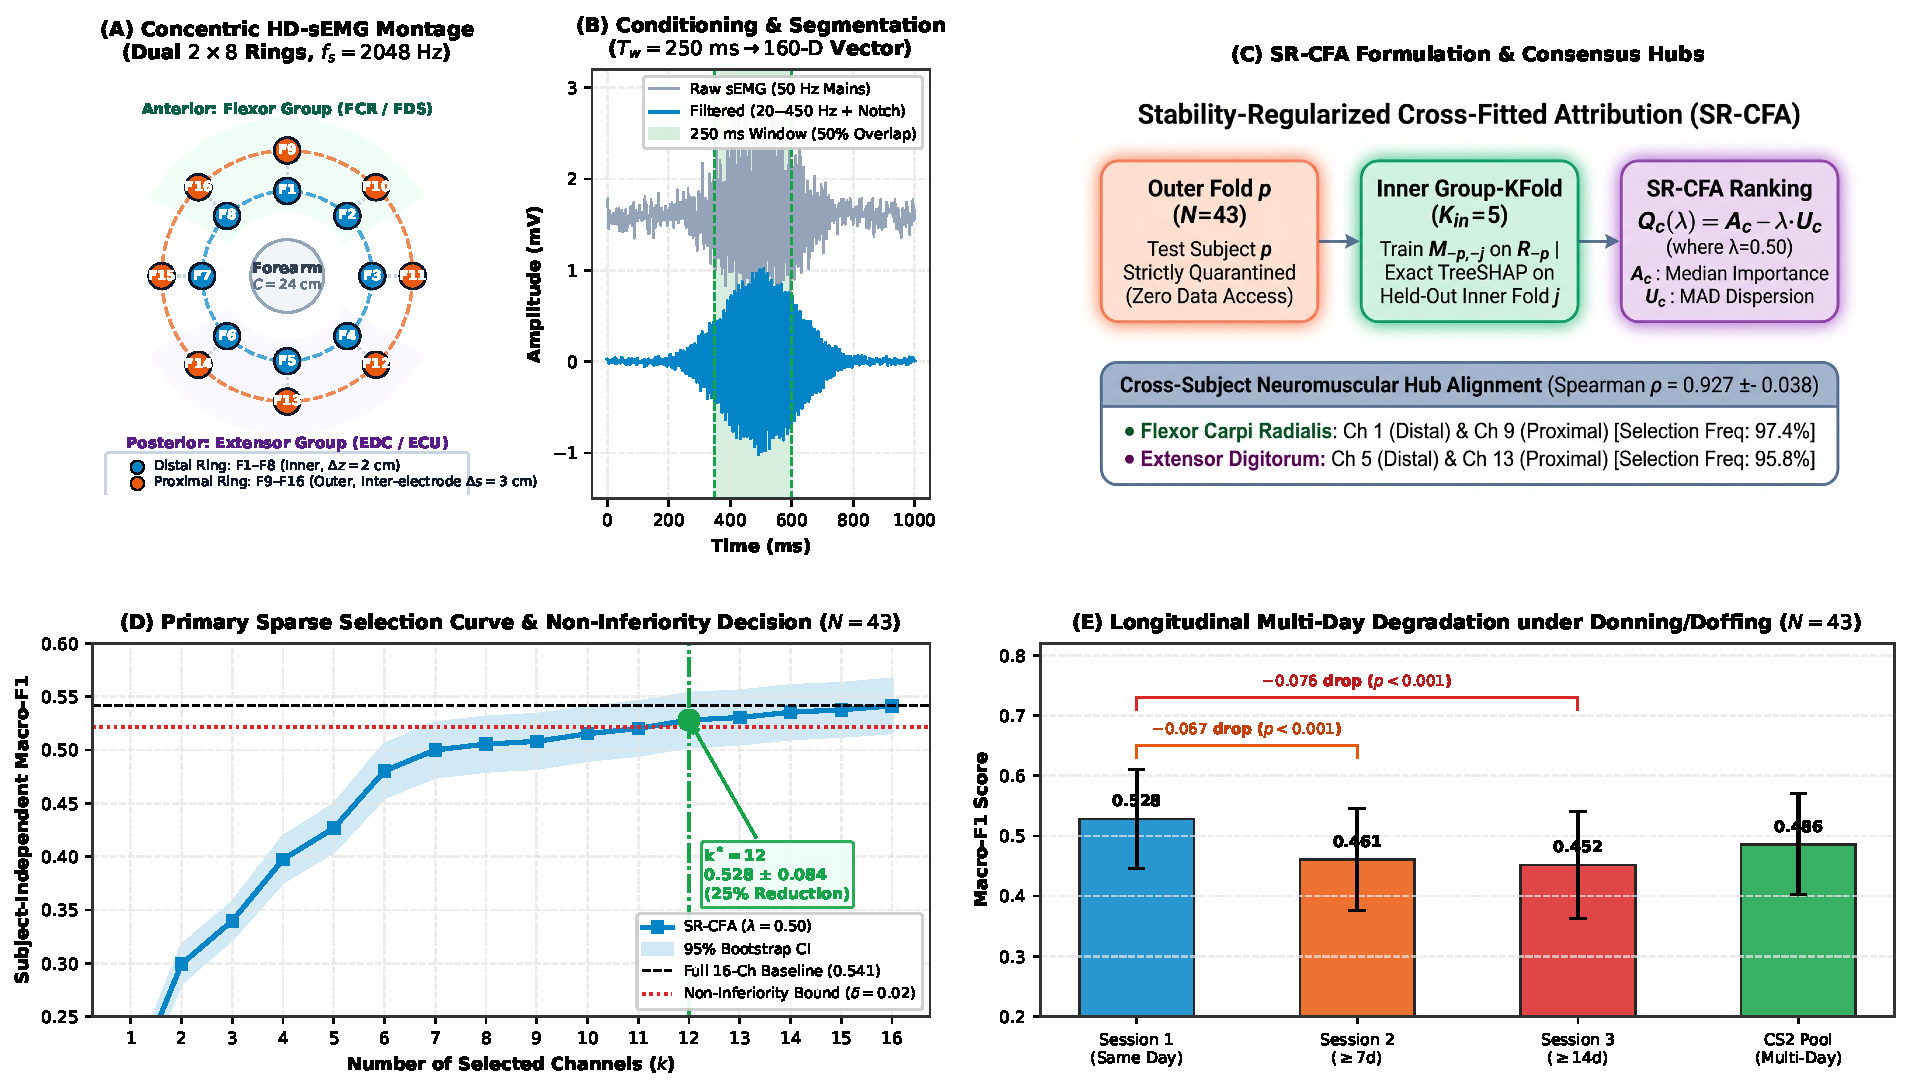
\includegraphics[height=0.58\textheight]{figures/fig1_workflow.pdf}
    \end{center}
    \vspace{-0.1cm}
    \scriptsize \textbf{Dòng chảy Logic:} (A) Bố trí vòng đôi $2 \times 8$ $\to$ (B) Lọc \& Trích xuất đặc trưng $\to$ (C) Khung SR-CFA không rò rỉ $\to$ (D) Kiểm định thống kê $k^*=12$ $\to$ (E) Thử thách tháo lắp đa ngày.
\end{frame}

% -----------------------------------------------------------------------------
% Slide 5: Method 1: Zero-Leakage LOSO & Cross-Fitting
% -----------------------------------------------------------------------------
\begin{frame}{4. Cơ Chế 1: Cách Ly Dữ Liệu Tuyệt Đối (Zero-Leakage Cross-Fitting)}
    \begin{columns}[T]
        \begin{column}{0.48\textwidth}
            \begin{block}{\textbf{Vòng Ngoài: Outer LOSO ($N=43$)}}
                \footnotesize
                \begin{itemize}
                    \item Trong mỗi lượt, \textbf{Người test $p$ bị cô lập 100\%} ở ngoài phòng thí nghiệm.
                    \item Tập huấn luyện chỉ gồm 42 người còn lại ($550{,}376$ cửa sổ tín hiệu).
                    \item Tuyệt đối không để thông tin người test lọt vào bước xếp hạng kênh.
                \end{itemize}
            \end{block}
        \end{column}
        
        \begin{column}{0.49\textwidth}
            \begin{exampleblock}{\textbf{Vòng Trong: Inner Cross-Fitting ($K_{\text{in}}=5$)}}
                \footnotesize
                \begin{itemize}
                    \item Chia 42 người huấn luyện thành 5 nhóm.
                    \item Mô hình huấn luyện trên 4 nhóm; tính điểm gán quyền TreeSHAP trên nhóm thứ 5 bị giữ lại.
                    \item \textbf{Nguyên tắc:} Không có mẫu dữ liệu nào tự chấm điểm cho chính mình $\to$ Triệt tiêu hoàn toàn thiên lệch XAI.
                \end{itemize}
            \end{exampleblock}
        \end{column}
    \end{columns}
\end{frame}

% -----------------------------------------------------------------------------
% Slide 6: Method 2: Mathematical Formulation of SR-CFA
% -----------------------------------------------------------------------------
\begin{frame}{5. Cơ Chế 2: Công Thức SR-CFA --- Thưởng Ổn Định, Phạt Biến Động}
    \begin{columns}[T]
        \begin{column}{0.48\textwidth}
            \begin{block}{\textbf{Các Bước Tính Điểm Từng Kênh}}
                \scriptsize
                \begin{enumerate}
                    \item \textbf{Gom cụm 10 đặc trưng:} $S_c^{(p,i)} = \sum_{f=1}^{10} \Phi_{c,f}^{(p,i)}$
                    \item \textbf{Xu hướng trung vị (Median Importance):}\\
                    $A_c = \text{median}_{i \in R_{-p}} (S_c^{(p,i)})$
                    \item \textbf{Độ phân tán cá nhân (MAD Dispersion):}\\
                    $U_c = \text{median}_{i \in R_{-p}} |S_c^{(p,i)} - A_c|$
                \end{enumerate}
            \end{block}
        \end{column}
        
        \begin{column}{0.49\textwidth}
            \begin{alertblock}{\textbf{Công Thức Điểm Ổn Định $Q_c(\lambda)$}}
                \small
                \[
                    \mathbf{Q_c(\lambda) = A_c - \lambda \cdot U_c} \quad (\lambda = 0.50)
                \]
            \end{alertblock}
            
            \begin{exampleblock}{\textbf{Giải thích Trực quan Dễ hiểu}}
                \scriptsize
                \begin{itemize}
                    \item \textbf{Thưởng $A_c$:} Kênh có khả năng phân loại cử chỉ cao.
                    \item \textbf{Phạt $\lambda U_c$:} Phạt nặng các kênh có phong độ thất thường (hôm nay quan trọng với người A nhưng vô dụng với người B do cấu trúc cơ khác nhau).
                    \item \textbf{$\lambda = 0.50$:} Đạt sự ổn định tối đa trên đối tượng mới.
                \end{itemize}
            \end{exampleblock}
        \end{column}
    \end{columns}
\end{frame}

% -----------------------------------------------------------------------------
% Slide 7: Method 3: Participant-Level Non-Inferiority
% -----------------------------------------------------------------------------
\begin{frame}{6. Cơ Chế 3: Kiểm Định Thống Kê Không Suy Giảm (Non-Inferiority)}
    \begin{columns}[T]
        \begin{column}{0.48\textwidth}
            \begin{block}{\textbf{Đặt Vấn Đề Thống Kê Y Khoa}}
                \footnotesize
                \begin{itemize}
                    \item Thay vì hỏi \textit{"Liệu ít kênh có giống hệt 16 kênh không?"}, ta hỏi theo chuẩn y tế:
                    \item \textbf{\textit{"Liệu sự suy giảm có nằm trong mức an toàn cho phép $\delta = 0.02$ ($2\%$) hay không?"}}
                    \item \textbf{Đơn vị phân tích:} Mức đối tượng ($N=43$), không gom cửa sổ đơn lẻ để giữ nguyên tương quan người.
                \end{itemize}
            \end{block}
        \end{column}
        
        \begin{column}{0.49\textwidth}
            \begin{exampleblock}{\textbf{Quy Tắc Quyết Định Tuyệt Đối $k^*$}}
                \footnotesize
                \begin{itemize}
                    \item Bootstrap phân cụm $B = 10{,}000$ lần trên 43 đối tượng.
                    \item Lấy cận dưới khoảng tin cậy $95\%$ ($\text{LCB}_{95\%}$):
                    \[
                        k^* = \min \left\{ k \in \{1,\dots,16\} \mid \text{LCB}_{95\%}(\Delta_k) > -\delta \right\}
                    \]
                    \item $k^*$ là số kênh nhỏ nhất chứng minh được \textbf{không thua kém mảng 16 kênh với độ tin cậy 95\%}.
                \end{itemize}
            \end{exampleblock}
        \end{column}
    \end{columns}
\end{frame}

% -----------------------------------------------------------------------------
% Slide 8: Empirical Results: Optimal k*=12 Decision
% -----------------------------------------------------------------------------
\begin{frame}{7. Kết Quả: Tìm Ra $k^*=12$ Kênh \& Khám Phá Về Giải Phẫu}
    \begin{columns}[T,onlytextwidth]
        \begin{column}{0.47\textwidth}
            \centering
            \resizebox{\linewidth}{!}{
            \begin{tabular}{ccccc}
                \toprule
                \textbf{Kênh ($k$)} & \textbf{Macro-F1} & $\mathbf{\bar{\Delta}_k}$ & $\mathbf{\text{LCB}_{95\%}}$ & \textbf{Kết luận} \\
                \midrule
                16 (Gốc) & $0.541 \pm 0.084$ & $0.0000$ & $0.0000$ & Tham chiếu \\
                15 & $0.537 \pm 0.085$ & $-0.0041$ & $-0.0064$ & Đạt chuẩn \\
                14 & $0.535 \pm 0.085$ & $-0.0062$ & $-0.0087$ & Đạt chuẩn \\
                13 & $0.530 \pm 0.084$ & $-0.0108$ & $-0.0135$ & Đạt chuẩn \\
                \textbf{12 ($k^*$)} & $\mathbf{0.528 \pm 0.084}$ & $\mathbf{-0.0133}$ & $\mathbf{-0.0160}$ & \textbf{Tối ưu ($> -0.02$)} \\
                11 & $0.520 \pm 0.084$ & $-0.0212$ & $-0.0253$ & \textbf{Bị loại ($\le -0.02$)} \\
                8  & $0.505 \pm 0.085$ & $-0.0359$ & $-0.0430$ & Bị loại \\
                6  & $0.480 \pm 0.084$ & $-0.0610$ & $-0.0713$ & Bị loại \\
                4  & $0.397 \pm 0.071$ & $-0.1440$ & $-0.1583$ & Bị loại \\
                \bottomrule
            \end{tabular}
            }
        \end{column}
        
        \begin{column}{0.50\textwidth}
            \begin{block}{\textbf{Ý Nghĩa Thực Tế \& Sinh Lý Cơ Bắp}}
                \scriptsize
                \begin{itemize}
                    \item \textbf{Giảm 25\% cảm biến ($k^*=12$):} Tiết kiệm đáng kể phần cứng mà vẫn giữ vững độ chính xác.
                    \item \textbf{Tại sao phải giữ 75\% kênh?} Bù đắp khác biệt giải phẫu cá nhân khi không hiệu chuẩn.
                    \item \textbf{Hai trạm trung chuyển Thần kinh - Cơ đối kháng:}
                    \begin{itemize}
                        \item \textbf{Cơ Gấp (FCR/FDS):} Kênh 1 (Xa) \& Kênh 9 (Gần) ($97.4\%$).
                        \item \textbf{Cơ Duỗi (EDC/ECU):} Kênh 5 (Xa) \& Kênh 13 (Gần) ($95.8\%$).
                        \item Độ ổn định xếp hạng Spearman đạt $\rho = 0.927 \pm 0.038$.
                    \end{itemize}
                \end{itemize}
            \end{block}
        \end{column}
    \end{columns}
\end{frame}

% -----------------------------------------------------------------------------
% Slide 9: Baseline Comparison Benchmark
% -----------------------------------------------------------------------------
\begin{frame}{8. Đọ Sức Thực Nghiệm với Các Thuật Toán Khác}
    \begin{center}
        \resizebox{0.92\textwidth}{!}{
        \begin{tabular}{lcccccc}
            \toprule
            \textbf{Số Kênh ($k$)} & \textbf{SR-CFA ($\lambda=0.5$)} & \textbf{Vanilla SHAP} & \textbf{Permutation} & \textbf{Mutual Info} & \textbf{Geometric} & \textbf{Random (500 lượt)} \\
            \midrule
            $k = 4$  & $0.383 \pm 0.071$ & $0.382 \pm 0.071$ & $\mathbf{0.385 \pm 0.070}$ & $0.280 \pm 0.049$ & $0.383 \pm 0.069$ & $0.366 \pm 0.059$ \\
            $k = 6$  & $\mathbf{0.453 \pm 0.080}$ & $\mathbf{0.453 \pm 0.080}$ & $0.440 \pm 0.080$ & $0.360 \pm 0.066$ & $0.419 \pm 0.068$ & $0.416 \pm 0.068$ \\
            $k = 8$  & $\mathbf{0.469 \pm 0.081}$ & $0.468 \pm 0.081$ & $0.466 \pm 0.080$ & $0.396 \pm 0.068$ & $0.465 \pm 0.072$ & $0.445 \pm 0.071$ \\
            $\mathbf{k = 12\ (k^*)}$ & $\mathbf{0.485 \pm 0.079}$ & $\mathbf{0.485 \pm 0.079}$ & $\mathbf{0.485 \pm 0.079}$ & $0.480 \pm 0.079$ & $0.478 \pm 0.076$ & $0.478 \pm 0.077$ \\
            \bottomrule
        \end{tabular}
        }
    \end{center}
    \vspace{0.05cm}
    \begin{columns}[T,onlytextwidth]
        \begin{column}{0.48\textwidth}
            \begin{block}{\textbf{Tại sao Mutual Information thất bại?}}
                \scriptsize
                \begin{itemize}
                    \item Mutual Info chỉ nhìn từng kênh riêng lẻ $\to$ Bỏ qua sự phối hợp đồng vận đa cơ ($0.360$ vs $0.453$ ở $k=6$).
                    \item SR-CFA luôn vượt trội hơn hẳn phân phối ngẫu nhiên (Random).
                \end{itemize}
            \end{block}
        \end{column}
        
        \begin{column}{0.48\textwidth}
            \begin{exampleblock}{\textbf{Giá trị của Tham số $\lambda = 0.50$}}
                \scriptsize
                \begin{itemize}
                    \item Triệt tiêu sự hỗn loạn của trọng số gán quyền giữa các cá nhân.
                    \item Mang lại một layout cảm biến thống nhất, dùng tốt cho người lạ.
                \end{itemize}
            \end{exampleblock}
        \end{column}
    \end{columns}
\end{frame}

% -----------------------------------------------------------------------------
% Slide 10: XAI Faithfulness Deletion Verification (ROAR)
% -----------------------------------------------------------------------------
\begin{frame}{9. Kiểm Chứng Tính Trung Thực: Thử Thách Xóa Kênh (ROAR)}
    \begin{columns}[T]
        \begin{column}{0.48\textwidth}
            \begin{block}{\textbf{Phép thử Vàng RemOve And Retrain}}
                \footnotesize
                Để chứng minh điểm số SHAP không phải là "ảo giác ngẫu nhiên", ta xóa kênh và huấn luyện lại từ đầu:
                \[
                    \mathbf{\text{F1}_{\text{xóa top}} \le \text{F1}_{\text{xóa ngẫu nhiên}} \le \text{F1}_{\text{xóa bottom}}}
                \]
                Xóa kênh quan trọng nhất $\to$ F1 phải tụt dốc thê thảm nhất!
            \end{block}
        \end{column}
        
        \begin{column}{0.49\textwidth}
            \begin{exampleblock}{\textbf{Bằng Chứng Thực Nghiệm Tuyệt Đối}}
                \scriptsize
                \begin{itemize}
                    \item \textbf{Khi giữ $k=12$ kênh (loại bỏ 4 kênh):}
                    \begin{itemize}
                        \item Xóa 4 kênh quan trọng nhất: F1 tụt xuống $\mathbf{0.488 \pm 0.079}$
                        \item Xóa 4 kênh ngẫu nhiên: F1 $= \mathbf{0.478 \pm 0.077}$
                        \item Xóa 4 kênh ít quan trọng nhất (giữ top 12): F1 $= \mathbf{0.528 \pm 0.084}$
                    \end{itemize}
                    \item \textbf{Khi giữ $k=6$ kênh (loại bỏ 10 kênh):}
                    \begin{itemize}
                        \item Xóa top: $\text{F1} = 0.399$ \quad | \quad Xóa bottom: $\text{F1} = 0.480$
                    \end{itemize}
                    \item \textbf{Kết luận:} Thứ tự bất đẳng thức được nghiệm đúng 100\%.
                \end{itemize}
            \end{exampleblock}
        \end{column}
    \end{columns}
\end{frame}

% -----------------------------------------------------------------------------
% Slide 11: Longitudinal Donning/Doffing & External Replication
% -----------------------------------------------------------------------------
\begin{frame}{10. Thử Thách Tháo Lắp Đa Ngày \& Kiểm Chứng Ngoại Vi}
    \begin{columns}[T]
        \begin{column}{0.48\textwidth}
            \begin{alertblock}{\textbf{Thách Thức Tháo Lắp Đa Ngày (Donning/Doffing)}}
                \scriptsize
                \begin{itemize}
                    \item \textbf{CS1 (Huấn luyện Ngày 1 $\to$ Thử nghiệm Ngày 2, 3):}
                    \begin{itemize}
                        \item Phiên 1 (Cùng ngày): $\text{F1} = 0.528 \pm 0.082$
                        \item Phiên 2 ($\ge 7\text{ ngày}$): $\text{F1} = 0.461$ (Sụt giảm $-0.067$)
                        \item Phiên 3 ($\ge 14\text{ ngày}$): $\text{F1} = 0.452$ (Sụt giảm $-0.076$)
                    \end{itemize}
                    \item \textbf{CS2 (Huấn luyện Ngày 1+2 $\to$ Thử nghiệm Ngày 3):}
                    \begin{itemize}
                        \item F1 hồi phục lên $\mathbf{0.486 \pm 0.084}$.
                        \item Dữ liệu đa ngày bù đắp độ lệch vị trí điện cực do tháo lắp.
                    \end{itemize}
                \end{itemize}
            \end{alertblock}
        \end{column}
        
        \begin{column}{0.49\textwidth}
            \begin{exampleblock}{\textbf{Nhân Bản Ngoại Kiểm NinaPro DB5 \& Vi Sai}}
                \scriptsize
                \begin{itemize}
                    \item \textbf{NinaPro DB5 ($N=10$ người, Myo $200\text{ Hz}$):}
                    \begin{itemize}
                        \item Mảng đầy đủ: $\text{F1} = 0.281 \pm 0.099$.
                        \item Điểm cắt $k=12$: $\text{F1} = 0.268 \pm 0.092$ ($\text{LCB} = -0.0200$, đúng mốc giữ $75\%$ kênh).
                        \item Kênh ưu tiên: Kênh 9, 16, 7, 6 (trùng khớp cơ gấp/duỗi).
                    \end{itemize}
                    \item \textbf{Cấu hình Vi Sai (Bipolar $N=43$):}
                    \begin{itemize}
                        \item Mảng 8 cặp vi sai: $\text{F1} = 0.471 \pm 0.090$.
                        \item Hội tụ chính xác vào các cặp vi sai đối kháng 6, 7, 5, 4.
                    \end{itemize}
                \end{itemize}
            \end{exampleblock}
        \end{column}
    \end{columns}
\end{frame}

% -----------------------------------------------------------------------------
% Slide 12: Summary & Translational Guidelines
% -----------------------------------------------------------------------------
\begin{frame}{11. Tổng Kết \& Khuyến Nghị Cho Kỹ Sư Thiết Kế Chi Giả}
    \begin{columns}[T]
        \begin{column}{0.48\textwidth}
            \begin{block}{\textbf{3 Đóng Góp Khoa Học Cốt Lõi}}
                \footnotesize
                \begin{enumerate}
                    \item \textbf{SR-CFA Framework:} Phương pháp gán quyền XAI không rò rỉ, ổn định cao, triệt tiêu phương sai cá nhân.
                    \item \textbf{Bằng chứng Non-Inferiority:} Xác lập điểm cắt toán học vững chắc $k^*=12$ (giảm $25\%$ cảm biến).
                    \item \textbf{Kiểm chứng toàn diện:} Đánh bại baseline, thỏa mãn ROAR, tái lập trên NinaPro DB5.
                \end{enumerate}
            \end{block}
        \end{column}
        
        \begin{column}{0.49\textwidth}
            \begin{exampleblock}{\textbf{3 Khuyến Nghị Thực Tế Thiết Kế Chi Giả}}
                \footnotesize
                \begin{itemize}
                    \item \textbf{Không giảm kênh cực đoan:} Phải giữ $\sim 75\%$ cảm biến nếu muốn chạy độc lập người dùng mà không cần hiệu chuẩn.
                    \item \textbf{Bố trí theo Hubs Thần kinh - Cơ:} Đặt cảm biến dày ở nhóm cơ gấp (FCR) và cơ duỗi (EDC).
                    \item \textbf{Thu thập dữ liệu đa ngày:} Huấn luyện trên ít nhất 2 ngày tháo lắp để chống suy giảm do trôi lệch vị trí.
                \end{itemize}
            \end{exampleblock}
        \end{column}
    \end{columns}
    
    \vspace{0.25cm}
    \begin{center}
        \footnotesize \textbf{\textcolor{vinNavy}{VinUniversity $\bullet$ Dữ liệu \& Đường ống Thực nghiệm Công khai 100\% Khả năng Tái Lập.}}
    \end{center}
\end{frame}

\end{document}
